\documentclass[tikz,border=2pt]{standalone}
\usepackage{amsmath}
\usepackage{pgfplots}
\pgfplotsset{compat=1.18}
\usetikzlibrary{arrows.meta}

\begin{document}
% At x0 the tangent line rises by dy = f'(x0) dx over a step dx, while the curve rises by
% Δy = f(x0+dx) - f(x0); the gap Δy - dy shrinks faster than dx.
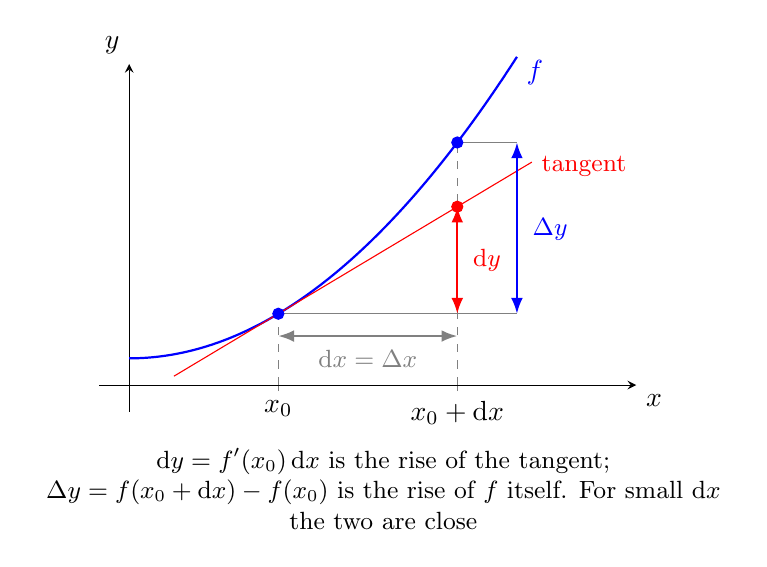
\begin{tikzpicture}
	\begin{axis}[
		axis lines=middle,
		xmin=-0.2, xmax=3.4,
		ymin=-0.3, ymax=3.6,
		xtick={1,2.2}, xticklabels={$x_0$,$x_0+\mathrm{d}x$},
		ytick=\empty,
		xlabel={$x$}, ylabel={$y$},
		xlabel style={below right}, ylabel style={above left},
		samples=100, smooth, clip=false,
		width=8.4cm, height=6cm
		]
		% f(x)=x^2/2+0.3, f(1)=0.8, f'(1)=1; f(2.2)=2.72; tangent at 2.2: 0.8+1.2=2.0
		\addplot[thick, blue, domain=0:2.6] {x^2/2+0.3};
		\addplot[red, domain=0.3:2.7] {x-0.2};
		\draw[dashed, gray] (axis cs:1,0) -- (axis cs:1,0.8);
		\draw[dashed, gray] (axis cs:2.2,0) -- (axis cs:2.2,2.72);
		\draw[gray] (axis cs:1,0.8) -- (axis cs:2.2,0.8);
		\draw[red, thick, {Latex[length=2mm]}-{Latex[length=2mm]}] (axis cs:2.2,0.8) -- (axis cs:2.2,2.0);
		\draw[blue, thick, {Latex[length=2mm]}-{Latex[length=2mm]}] (axis cs:2.6,0.8) -- (axis cs:2.6,2.72);
		\draw[gray] (axis cs:2.2,2.72) -- (axis cs:2.6,2.72);
		\draw[gray] (axis cs:2.2,0.8) -- (axis cs:2.6,0.8);
		\draw[gray, thick, {Latex[length=2mm]}-{Latex[length=2mm]}] (axis cs:1,0.55) -- (axis cs:2.2,0.55);
		\node[gray, anchor=north, font=\small] at (axis cs:1.6,0.5) {$\mathrm{d}x=\Delta x$};
		\node[red, anchor=west, font=\small] at (axis cs:2.24,1.4) {$\mathrm{d}y$};
		\node[blue, anchor=west, font=\small] at (axis cs:2.64,1.75) {$\Delta y$};
		\addplot[only marks, mark=*, blue] coordinates {(1,0.8) (2.2,2.72)};
		\addplot[only marks, mark=*, red] coordinates {(2.2,2.0)};
		\node[blue, anchor=west] at (axis cs:2.6,3.5) {$f$};
		\node[red, anchor=west, font=\small] at (axis cs:2.7,2.45) {tangent};
	\end{axis}
	\node[anchor=north, font=\small, align=flush center, text width=8.8cm] at ([yshift=-2pt]current axis.outer south) {$\mathrm{d}y=f'(x_0)\,\mathrm{d}x$ is the rise of the tangent; $\Delta y=f(x_0+\mathrm{d}x)-f(x_0)$ is the rise of $f$ itself. For small $\mathrm{d}x$ the two are close};
\end{tikzpicture}
\end{document}
